\documentclass{report}
\usepackage[utf8]{inputenc}
\usepackage{graphicx,setspace,csquotes}
\usepackage[T1]{fontenc}
\usepackage[skip=12pt, indent=30pt]{parskip}
\usepackage[english]{babel}
\usepackage{listings}
\usepackage{amsmath}
\usepackage[autolanguage]{numprint}
\usepackage[backend=biber,style=apa,sorting=nyt]{biblatex}
\usepackage[font=small,labelfont=bf]{caption}
% \usepackage[margin=2.5cm]{geometry}
\usepackage{booktabs}
\usepackage[english]{algorithm2e}
\usepackage{float}
\usepackage{hyperref}
\def\englishtablename{Tableau}
\usepackage{caption}
\usepackage{subcaption}
\usepackage{amssymb} 
\usepackage{xcolor}
%\usepackage{fancyhdr}
%\usepackage{enumitem}

% Configuration des liens
%New colors defined below
\definecolor{codegreen}{rgb}{0,0.6,0}
\definecolor{codegray}{rgb}{0.5,0.5,0.5}
\definecolor{codepurple}{rgb}{0.58,0,0.82}
\definecolor{backcolour}{rgb}{0.95,0.95,0.92}

\lstdefinestyle{mystyle}{
    backgroundcolor=\color{backcolour},   
    commentstyle=\color{codegreen},
    keywordstyle=\color{magenta},
    numberstyle=\tiny\color{codegray},
    stringstyle=\color{codepurple},
    basicstyle=\ttfamily\footnotesize,
    breakatwhitespace=false,         
    breaklines=true,                 
    captionpos=b,                    
    keepspaces=true,                 
    numbers=left,                    
    numbersep=5pt,                  
    showspaces=false,                
    showstringspaces=false,
    showtabs=false,                  
    tabsize=2
}

%"mystyle" code listing set
\lstset{style=mystyle}
\hypersetup{
    colorlinks=true,
    linkcolor=black,
    filecolor=black,      
    urlcolor=blue,
    citecolor=black,
    pdftitle={Report},
    pdfpagemode=FullScreen,
    }
\urlstyle{same}
% Configuration des algorithmes
% \RestyleAlgo{ruled}
% \SetKw{KwBy}{by}
% Configuration des légendes
\captionsetup{width=13.5cm}









\title{Research for Steamboat Willie's Store in Poland}
\author{Type your name} %% Remember this thing
\date{\today}


%date{September 2023}




%%% MAIN DOCUMENT START FROM HERE %%%%%%%%%%%%%%%%%%%
\begin{document}

\maketitle 
% \newpage
 \tableofcontents
 % \newpage
 \listoffigures
\newpage
% \listoflistings
% \renewcommand\listoflistingscaption{List of source codes}
% \listoflistings
% \newpage




\chapter{Preliminary Research for Steamboat Willie's in Poland}
\section*{Introduction}
The new fast-food chain, Steamboat Willie's, is planning to expand its presence in Poland. This report presents preliminary research conducted to determine the number of stores required to ensure that every town in Poland has a Steamboat Willie's within a 50km radius.
\section*{Data Analysis}
The dataset used for this research consists of information about cities in Poland and other countries as well, including their geographical coordinates. The data was preprocessed to extract relevant information.

\begin{center}
    \begin{lstlisting}[language=Python, caption=Loading the Dataset]
    import pandas as pd

# Specify the path to your local JSON file
# The dataset given as json file
file_path = r"C:\Users\Perpendicooler\Downloads\dataset.json"


# Read the JSON file into a DataFrame
df = pd.read_json(file_path)
# Save the DataFrame to an Excel file
# We save the dataframe into an excel file for better view
df.to_excel('output.xlsx', index=False)

#files.download('output.xlsx')

# Display the first few rows of the DataFrame
df.head()

\end{lstlisting}
\end{center}
The Python code filters a DataFrame (\texttt{df}) to extract data related to Poland (\texttt{'cou\_name\_en' == 'Poland'}). The filtered data is stored in a new DataFrame called \texttt{poland\_data}. The code then prints the filtered DataFrame and exports the entire original DataFrame to an Excel file ('output\_with\_poland.xlsx').
\begin{center}
    \begin{lstlisting}[language=Python, caption=Loading the Dataset]
        poland_data = df[df['cou_name_en'] == 'Poland'].copy()

# Display the filtered DataFrame
print(poland_data)
df.to_excel('output_with_poland.xlsx', index=False)

    \end{lstlisting} 
\end{center} 
The Python code reads an Excel file located at local pc into a DataFrame (\texttt{df}) using the \texttt{pd.read\_excel()} function. The data is assumed to be manipulated for improvement. Subsequently, it prints the contents of the DataFrame.
\begin{center}
    \begin{lstlisting}[language=Python, caption=Loading the Dataset]
        file_path_poland = r"C:\Users\Perpendicooler\manupulated_data.xlsx"
df = pd.read_excel(file_path_poland)
print(df)
    \end{lstlisting}
\end{center}
The Python code calculates pairwise distances between the first 500 cities in Poland using their latitude and longitude coordinates. It uses the Haversine formula to compute distances on the Earth's surface. The dataset is loaded from a JSON file ('dataset.json'), and relevant columns are extracted for cities in Poland. The computed distances are then stored in an Excel file.
\begin{center}
    \begin{lstlisting}[language=Python, caption=Loading the Dataset]
    import itertools
import pandas as pd
from sklearn.metrics.pairwise import haversine_distances
from math import radians

def distance(row1, row2):
    pos1 = (row1['coordinates']['lat'], row1['coordinates']['lon'])
    pos2 = (row2['coordinates']['lat'], row2['coordinates']['lon'])
    radians1 = [radians(pos1[0]), radians(pos1[1])]
    radians2 = [radians(pos2[0]), radians(pos2[1])]
    res = haversine_distances([radians1, radians2])
    res *= 6371000 / 1000  # multiply by Earth radius to get kilometers
    return res[0][1]

# Load the dataset
df = pd.read_json("dataset.json")

# Extract relevant columns for the first 500 cities in Poland
# We can extract any number of city just we need to change the 500 in this with any number i want.
poland_data = df[df['country_code'] == 'PL'].head(500)[['name', 'coordinates']]

# Initialize an empty list to store pairs of cities and distances
distances = []

# Iterate through each pair of cities in the first 50 cities in Poland
for (city1_idx, city1), (city2_idx, city2) in itertools.combinations(poland_data.iterrows(), 2):
    dist = distance(city1, city2)
    
    # Append the pair and distance to the list
    distances.append((city1['name'], city2['name'], dist))

# Create a dataframe from the distances
distance_df = pd.DataFrame(distances, columns=['From', 'To', 'Distance'])

# Store the distances in an Excel file
distance_df.to_excel('poland_500_cities_pairwise_distances.xlsx', index=False)

        
    \end{lstlisting}
\end{center}
The Python code calculates pairwise distances between 50 cities in Poland using their latitude and longitude coordinates to optimize computation time. The Haversine formula is employed for distance calculation on the Earth's surface. Instead of processing all 500 cities, a subset of 10 cities is chosen for demonstration purposes, allowing the program to run more efficiently. The dataset is loaded from a JSON file ('dataset.json'), and relevant columns are extracted. The computed distances are then stored in an Excel file in local machine.
\newpage
\section*{Optimized Result}
Using integer programming to computed the number of  stores does STEAMBOAT WILLIE's need to open for the restriction of 50km, as above.

\begin{center}
    \begin{lstlisting}[language=Python, caption=Minimize the store opening within 50km in every city of poland]
        import pandas as pd
from pulp import LpVariable, LpProblem, LpMinimize, lpSum

# Load data from Excel
data = pd.read_excel(r"C:\Users\Perpendicooler\poland_50_cities_pairwise_distances.xlsx")  

# Extract city names and distances
city_names = set(data["From"].tolist() + data["To"].tolist())
city_index = {city: i for i, city in enumerate(city_names)}
distances = {}
for row in data.itertuples():
    distances[(city_index[row.From], city_index[row.To])] = row.Distance

# Set the coverage radius
coverage_radius = 50

# Create optimization model
model = LpProblem("StorePlacement", LpMinimize)

# Decision variables: whether to open a store in each city
s = {i: LpVariable(name=f"store_{i}", cat="Binary") for i in range(len(city_names))}

# Objective: Minimize the total number of stores opened
model += lpSum(s), "Minimize Stores"

# Constraint: Every city must have at least one store within 50km
for city in range(len(city_names)):
    model += lpSum(s[j] for j in range(len(city_names)) if city != j and (city, j) in distances) >= 1, f"City {city+1} Coverage"

# Solve the model
model.solve()

# Analyze results
num_stores = int(model.objective.value())

# Print the cities where the stores are opened
print("Open stores:")
for i, city in enumerate(city_names):
    if int(s[i].value()) == 1:
        print(f"{city}")

# Check coverage and open additional stores if needed
while True:
    coverage = {city: False for city in city_names}
    
    # Check coverage for each city
    for i, city in enumerate(city_names):
        if int(s[i].value()) == 1:
            coverage[city] = True
            for j in range(len(city_names)):
                if city != j and (city, j) in distances and distances[(city, j)] > coverage_radius:
                    coverage[city] = False
    
    # If any city is not covered within 50km range, open a new store in the uncovered city
    if False in coverage.values():
        uncovered_city = next(city for city, covered in coverage.items() if not covered)
        model += s[city_index[uncovered_city]] == 1
        model.solve()
        num_stores += 1
        print(f"{uncovered_city}")
    else:
        break

print(f"Final number of stores needed: {num_stores}")
# Create a DataFrame with the results
results_df = pd.DataFrame(index=range(1, len(city_names) + 1), columns=["City Name"])

# Populate the DataFrame with the cities where stores are opened
for i, city in enumerate(city_names):
    if int(s[i].value()) == 1:
        results_df.at[i+1, "City Name"] = city

# Save the results to an Excel file
results_df.to_excel("opened_stores_results.xlsx", index_label="Index")


    \end{lstlisting}
\end{center}


The optimization model aims to minimize the number of stores opened in a set of cities within a coverage radius of 50 km. The initial solution opens stores in several cities, and the algorithm iteratively checks the coverage and opens additional stores if necessary.

\subsection*{Opened Stores}

\begin{verbatim}
Open stores:
Borowa
Sawin
...
Wiśniowa
Krynki
Aleksandrów Łódzki
Jodłówka-Wałki
\end{verbatim}

\subsection*{Final Number of Stores Needed}

\begin{verbatim}
Final number of stores needed: 115
\end{verbatim}

\subsection*{Results DataFrame}
We need to open 115 stores in order to cover all the city.
So that everyone from any city can access to that store within 50km. The opened stores' information is saved in a DataFrame and stored in an Excel file named 'opened\_stores\_results.xlsx'.
\section*{ Minimum Distances for Different Store Counts}

Suppose the correct answer is 115. The table below shows the minimum distance $D$ for each scenario of opening exactly $k \leq 115$ stores, ensuring that every town in Poland can have a STEAMBOAT WILLIE'S within $D$ km.
\begin{center}
    \begin{lstlisting}[language=Python, caption=Minimum Resturent we need to open]
        import pandas as pd
from pulp import LpProblem, LpVariable, lpSum, LpMinimize, LpStatus

# Load data from Excel
data = pd.read_excel(r"C:\Users\Perpendicooler\poland_50_cities_pairwise_distances.xlsx")  

# Extract city names and distances
city_names = set(data["From"].tolist() + data["To"].tolist())
city_index = {city: i for i, city in enumerate(city_names)}
distances = {(city_index[row.From], city_index[row.To]): row.Distance for row in data.itertuples()}

# Set the maximum number of stores
max_stores = 115

# Create a DataFrame to store results
results_df = pd.DataFrame(index=range(1, max_stores + 1), columns=["Number of Stores", "Minimum Distance"])

# Iterate over the number of stores (k)
for k in results_df.index:
    # Create optimization model
    model = LpProblem("StorePlacement", LpMinimize)

    # Decision variables: whether to open a store in each city
    s = {i: LpVariable(name=f"store_{i}", cat="Binary") for i in range(len(city_names))}

    # Objective: Minimize the total distance
    model += lpSum(distances[i, j] * s[i] for i in range(len(city_names)) for j in range(len(city_names)) if (i, j) in distances), "Minimize Distance"

    # Constraint: Open exactly k stores
    model += lpSum(s[i] for i in range(len(city_names))) == k, f"OpenExactly_{k}_Stores"

    # Solve the model
    model.solve()

    # Store the results in the DataFrame
    results_df.at[k, "Number of Stores"] = k
    results_df.at[k, "Minimum Distance"] = lpSum(distances[i, j] * s[i].value() for i in range(len(city_names)) for j in range(len(city_names)) if (i, j) in distances).value()

# Display the results table
print(results_df)
results_df.to_excel("store_placement_results.xlsx", index_label="Index")

    \end{lstlisting}
\end{center}

\begin{table}[h]
\centering
\begin{tabular}{ccc}
\toprule
\textbf{Number of Stores ($k$)} & \textbf{Minimum Distance ($D$)} & \\
\midrule
1 & ... & \\
2 & ... & \\
3 & ... & \\
... & ... & \\
115 & ... & \\
\bottomrule
\end{tabular}
\caption{Minimum Distances for Different Store Counts}
\end{table}

\section*{ Linear Programming Relaxation}
Finally, we compute the linear programming relaxation of the integer programming problem. This involves determining how many stores need to be opened, allowing for fractions of stores in cities, so that every town in Poland has at least one within 50 km.

The linear programming relaxation problem can be expressed as follows:

\begin{align*}
\text{Minimize} & \quad \text{Total Stores} \\
\text{Subject to} & \quad \text{Coverage Constraint for each city within 50 km} \\
& \quad \text{Fractional store opening variables} \in [0, 1] \\
\end{align*}
\newpage
\begin{center}
    \begin{lstlisting}[language=Python, caption=linear programming relaxation]
        import pandas as pd
from pulp import LpProblem, LpVariable, lpSum, LpMinimize, LpStatus

# Load data from Excel
data = pd.read_excel(r"C:\Users\Perpendicooler\poland_50_cities_pairwise_distances.xlsx")  # Replace with your actual file path

# Extract city names and distances
city_names = set(data["From"].tolist() + data["To"].tolist())
city_index = {city: i for i, city in enumerate(city_names)}
distances = {(city_index[row.From], city_index[row.To]): row.Distance for row in data.itertuples()}

# Create optimization model for linear programming relaxation
model_relaxation = LpProblem("StorePlacementRelaxation", LpMinimize)

# Decision variables: fraction of a store to open in each city
s_relaxation = {i: LpVariable(name=f"store_{i}", lowBound=0, upBound=1) for i in range(len(city_names))}

# Objective: Minimize the total distance
model_relaxation += lpSum(distances[i, j] * s_relaxation[i] for i in range(len(city_names)) for j in range(len(city_names)) if (i, j) in distances), "Minimize Distance"

# Constraint: Every city must have at least one store within 50km
for city in range(len(city_names)):
    model_relaxation += lpSum(distances[i, j] * s_relaxation[i] for i in range(len(city_names)) for j in range(len(city_names)) if (i, j) in distances and i != j) >= 1, f"City {city+1} Coverage"

# Solve the model
model_relaxation.solve()

# Display the results
print("Status:", LpStatus[model_relaxation.status])
rounded_stores_needed = round(model_relaxation.objective.value())
print("Number of stores needed (fractional):",model_relaxation.objective.value())
print("Number of stores needed (rounded):", rounded_stores_needed)

    \end{lstlisting}
\end{center}
\newpage
\subsection*{Results Data Frame}
\begin{verbatim}
Status: Optimal
Number of stores needed (fractional): 0.999999981492213
Number of stores needed (rounded): 1
\end{verbatim}
The output indicates that the linear programming relaxation of the integer programming problem has been solved, and the solution is optimal. The fractional solution suggests that a minimum of approximately 1 store is needed to meet the coverage constraints for every town in Poland, with each store contributing a fraction of its presence.



\chapter{Exploring TSP: Integer LP Formulation and Lazy Row Generation}
\section*{Introduction}

The Metric Traveling Salesman Problem (TSP) is a classic optimization problem where the goal is to find the shortest possible tour that visits a set of points exactly once. This report presents the implementation and results of two approaches for solving the metric TSP problem: the Integer Linear Programming (LP) formulation with exponentially many constraints, and a "lazy row generation" version.

\section*{Integer LP Formulation}

The first approach involves implementing the Integer LP formulation, specifically the Dantzig-Fulkerson-Johnson formulation as described in \cite{dfj-formulation}. This formulation typically includes exponentially many constraints, making it challenging for large instances.
\newpage
\subsection*{Implementation}

The Integer LP formulation was implemented using pandas and lp, and the provided dataset is 50-cities-pairwise-distance.We manipulate the data as to make a Source and destination and cost vector. By making a symmetric matrix out of it.
\begin{center}
    \begin{lstlisting}[language = Python]
        import pandas as pd

# Load data from Excel we can take any number of cities_pairwise 
df = pd.read_excel(r"C:\Users\Perpendicooler\poland_50_cities_pairwise_distances.xlsx")

# Create a list of unique city names
cities = list(set(df['From'].tolist() + df['To'].tolist()))

# Create a pivot table to organize distances
distance_matrix = df.pivot_table(values='Distance', index='From', columns='To', aggfunc='first')

# Ensure symmetry
distance_matrix = distance_matrix.add(distance_matrix.T, fill_value=0)

# Explicitly set diagonal to zeros
for city in cities:
    distance_matrix.at[city, city] = 0

# Save the distance matrix to a new Excel file
distance_matrix.to_excel(r"C:\Users\Perpendicooler\distance_matrix.xlsx")

# Display the distance matrix
print("Distance Matrix:")
print(distance_matrix)

    \end{lstlisting}
\end{center}
Now We will excute the program for this distance matrix to find the best possible outcome for TSP.
\begin{center}
\begin{lstlisting}[language=Python, caption={Integer LP Formulation Implementation}]
import pandas as pd
from pulp import LpProblem, LpVariable, lpSum, LpMinimize, LpStatus

# Load data from Excel, setting 'Unnamed: 0' as the index
data = pd.read_excel(r"C:\Users\Perpendicooler\distance_matrix.xlsx", index_col='Unnamed: 0')

# Extract city names
city_names = list(data.columns)
city_indices = {city: i for i, city in enumerate(city_names)}

# Extract distances
distances = {(city_indices[i], city_indices[j]): data.at[i, j] for i in city_names for j in city_names if i != j}

# Create optimization model
model_tsp = LpProblem("TSP", LpMinimize)

# Decision variables
x = {(i, j): LpVariable(name=f"x_{i}_{j}", cat='Binary') for i in city_indices.values() for j in city_indices.values() if i != j}

# Objective function
model_tsp += lpSum(distances[i, j] * x[i, j] for i in city_indices.values() for j in city_indices.values() if i != j), "Minimize Distance"

# Constraints
# Ensure that each city is visited exactly once
for i in city_indices.values():
    model_tsp += lpSum(x[i, j] for j in city_indices.values() if i != j) == 1, f"VisitOnce_{i}"

# Ensure that each city is left exactly once
for j in city_indices.values():
    model_tsp += lpSum(x[i, j] for i in city_indices.values() if i != j) == 1, f"LeaveOnce_{j}"


# Solve the model
model_tsp.solve()

# Display the results
print("Status:", LpStatus[model_tsp.status])

# Print the optimal path
optimal_path = [var for var in model_tsp.variables() if var.value() == 1]
print("Optimal Path:")
for var in sorted(optimal_path, key=lambda v: (int(v.name.split('_')[1]), int(v.name.split('_')[2]))):
    print(f"{var.name}: {var.value()}")
    
def get_city_name(index):
    return next(city for city, idx in city_indices.items() if idx == index)

# Display the optimal path
optimal_path_indices = [int(var.name.split('_')[1]) for var in optimal_path]
optimal_path_indices.append(optimal_path_indices[0])  # Add the starting city at the end to complete the loop

optimal_path_names = [get_city_name(idx) for idx in optimal_path_indices]

print("Optimal Path:")
print(" -> ".join(optimal_path_names))    


\end{lstlisting}
    
\end{center}

\subsection*{Results}
The provided sequence is a solution to the Traveling Salesman Problem (TSP) for a given set of cities. In TSP, the goal is to find the shortest possible tour that visits each city exactly once and returns to the starting city. The sequence you provided represents an optimal tour that minimizes the overall travel distance for the specified cities. The TSP solution starts and ends in "Aleksandrów Łódzki" and traverses through the listed cities in the order mentioned.\newline\newline
\texttt{
Optimal Path:
Aleksandrów Łódzki -> Daszyna -> Dobre Miasto -> Dwikozy -> Dziekanów Leśny -> Dąbie -> Firlej -> Godziszów -> Grójec -> Hrubieszów -> Iłża -> Biały Bór -> Jakubów -> Jastków -> Jodłówka-Wałki -> Józefów nad Wisłą -> Karczmiska -> Korczew -> Krasnopol -> Krynki -> Krzywda -> Maszkienice -> Borowa -> Niedźwiada -> Opatów -> Ostrów -> Paprotnia -> Pruchnik -> Raczki -> Radoszyce -> Rejon ulicy Saperów -> Rzgów -> Sawin -> Cegłów -> Siedliska -> Srokowo -> Swojczyce -> Szarów -> Wiśniowa -> Wyśmierzyce -> Wólka Tanewska -> Węgorzewo -> Łapy -> Żurowa -> Cewice -> Chmielnik -> Ciepielów -> Czarków -> Czarna Woda -> Człopa -> Aleksandrów Łódzki
}

\section*{Lazy Row Generation}

The second approach involves a "lazy row generation" version, where constraints are added progressively until a valid tour is found. This method is known for its efficiency in solving large instances.

\subsection*{Implementation}

The lazy row generation version was implemented using [solver/library], with inspiration from the Gurobi example \href{https://colab.research.google.com/github/Gurobi/modeling-examples/blob/master/traveling_salesman/tsp.ipynb}{\textbf{Gurobi-example}} 
\subsection*{Data computation}The following function calculates the distance for 50 each pair of cities. Since we are solving the symmetric traveling salesman problem, we use combinations of cities.

\begin{lstlisting}[language=Python, caption={Data Computation}]
import pandas as pd

# Replace 'your_file.xlsx' with the path to your Excel file
file_path = r"C:\Users\Perpendicooler\poland_50_cities_pairwise_distances.xlsx"

# Read the Excel file into a DataFrame
df = pd.read_excel(file_path)

# Display the DataFrame
print(df)
\end{lstlisting}
\subsection*{Model Code}
We now write the model for the TSP, by defining decision variables, constraints, and objective function. Because this is the symmetric traveling salesman problem, we can make it more efficient by setting the object x[j,i] to x[i,j], instead of a constraint
\begin{center}
    \begin{lstlisting}[language=Python, caption={Optimize the Model}]
    import pandas as pd
import gurobipy as gp
from gurobipy import GRB

# Load data from Excel
file_path = r"C:\Users\Perpendicooler\poland_50_cities_pairwise_distances.xlsx"
data = pd.read_excel(file_path)

# Extract city names and distances
cities = set(data["From"].tolist() + data["To"].tolist())
city_index = {city: i for i, city in enumerate(cities)}
distances = {(city_index[row.From], city_index[row.To]): row.Distance for row in data.itertuples()}

# Create a Gurobi model
m = gp.Model()

# Variables: is city 'i' adjacent to city 'j' on the tour?
vars = m.addVars(distances.keys(), obj=distances, vtype=GRB.BINARY, name='x')

# Symmetric direction: Copy the object
keys = list(vars.keys())  # Create a list of keys
for i, j in keys:
    vars[j, i] = vars[i, j]  # edge in opposite direction

# Constraints: two edges incident to each city
capitals = [i for i in range(len(cities))]
cons = m.addConstrs(vars.sum(c, '*') == 2 for c in capitals)

# Optimize the model
m.optimize()

# Print the tour
tour = [i for i, j in vars.keys() if vars[i, j].X > 0.5]
print("Tour:", tour)

        
    \end{lstlisting}
\end{center}

\subsection*{Results}
\begin{verbatim}
olution count 4: 2698.1 2786.02 2810.06 13005.3 
Optimal solution found (tolerance 1.00e-04)
Best objective 2.698101399109e+03, best bound 2.698101399109e+03, gap 0.0000%
\end{verbatim}
\subsection*{Callback}
\begin{center}
    \begin{lstlisting}[language=Python, caption={Using Callback Function}]
        # Callback - use lazy constraints to eliminate sub-tours
def subtourelim(model, where):
    if where == GRB.Callback.MIPSOL:
        # make a list of edges selected in the solution
        vals = model.cbGetSolution(model._vars)
        selected = gp.tuplelist((i, j) for i, j in model._vars.keys() if vals[i, j] > 0.5)
        # find the shortest cycle in the selected edge list
        tour = subtour(selected)
        if len(tour) < len(capitals):
            # add subtour elimination constr. for every pair of cities in subtour
            model.cbLazy(gp.quicksum(model._vars[i, j] for i, j in combinations(tour, 2)) <= len(tour) - 1)

# Given a tuplelist of edges, find the shortest subtour
def subtour(edges):
    unvisited = capitals[:]
    cycle = capitals[:]  # Dummy - guaranteed to be replaced
    while unvisited:  # true if list is non-empty
        thiscycle = []
        neighbors = unvisited
        while neighbors:
            current = neighbors[0]
            thiscycle.append(current)
            unvisited.remove(current)
            neighbors = [j for i, j in edges.select(current, '*') if j in unvisited]
        if len(thiscycle) <= len(cycle):
            cycle = thiscycle  # New shortest subtour
    return cycle

# Set the callback function
m._vars = vars
m.Params.LazyConstraints = 1
m.optimize(subtourelim)

    \end{lstlisting}
\end{center}
\newpage
\subsection*{Results For callback}
\begin{verbatim}
  Solution count 4: 2698.1 2786.02 2810.06 13005.3 

Optimal solution found (tolerance 1.00e-04)
Best objective 2.698101399109e+03, best bound 2.698101399109e+03, gap 0.0000%

User-callback calls 30, time in user-callback 0.00 sec  
\end{verbatim}


\section*{Conclusion}

In conclusion, the report outlines the implementation and results of two approaches for solving the metric TSP problem. The Integer LP formulation with exponentially many constraints and the lazy row generation version were explored, with each having its strengths and limitations. Further analysis and experimentation may be conducted to improve the scalability and efficiency of both methods.



\chapter{Comparative Analysis of Christofides Algorithm and ILP Solutions for Metric TSP}
\section*{Introduction}
The Christofides algorithm is a well-known approximation algorithm for solving the Metric Traveling Salesman Problem (TSP). This report presents the implementation and performance comparison of the Christofides algorithm against the optimal Integer Linear Programming (ILP) solutions obtained in Task 2.

\section*{Implementation of Christofides Algorithm}
The Christofides algorithm was implemented to approximate the metric TSP on a chosen subset of the dataset stored in distance-matrix.xlsx. The main challenge lies in finding a library for perfect matching of minimum cost, a crucial step in the Christofides algorithm. 

\begin{lstlisting}[language=Python, caption={Christofides Algorithm Implementation}]
import pandas as pd
import networkx as nx
import matplotlib.pyplot as plt
from itertools import permutations
from scipy.spatial.distance import euclidean
from scipy.optimize import linear_sum_assignment
import time
from pulp import LpProblem, LpVariable, lpSum, LpMinimize, LpStatus

# Step 1: Read the data from Excel
file_path = r"C:\Users\Perpendicooler\distance_matrix.xlsx"
df = pd.read_excel(file_path, index_col=0)

# Step 2: Create a graph from the distance matrix for Christofides algorithm
G_christofides = nx.Graph()
cities = df.index
G_christofides.add_nodes_from(cities)

for i, j in permutations(cities, 2):
    G_christofides.add_edge(i, j, weight=df.at[i, j])

# Step 3: Solve TSP using the Christofides algorithm
start_time_christofides = time.time()

# Approximation algorithm
approximate_tour_christofides = nx.approximation.traveling_salesman_problem(G_christofides, weight="weight", cycle=True)

# Compute the total distance of the approximate tour
approximate_tour_length_christofides = sum(G_christofides[i][j]["weight"] for i, j in zip(approximate_tour_christofides, approximate_tour_christofides[1:]))

end_time_christofides = time.time()

# Step 4: Print the results for Christofides algorithm
print("Approximate tour length (Christofides):", approximate_tour_length_christofides)
print("Approximate tour (Christofides):", approximate_tour_christofides)

# Step 5: Plot the graph with the approximate tour for Christofides algorithm
pos_christofides = nx.spring_layout(G_christofides)
nx.draw(G_christofides, pos_christofides, with_labels=True, font_weight="bold")
edges_christofides = list(zip(approximate_tour_christofides, approximate_tour_christofides[1:]))
nx.draw_networkx_edges(G_christofides, pos_christofides, edgelist=edges_christofides, edge_color="r", width=2)
plt.title('Christofides Algorithm')
plt.savefig('christofides_plot.png')
plt.show()
\end{lstlisting}
\newpage
\subsection*{Results}
\subsection*{Approximate Tour using Christofides Algorithm}

The Christofides algorithm was employed to solve the Traveling Salesman Problem on the given dataset. The approximate tour length achieved is 3002.15 units.\newline
The approximate tour path is as follows:
\[
\begin{aligned}
&\text{['Aleksandrów Łódzki', 'Daszyna', 'Dąbie', 'Swojczyce', 'Rejon ulicy Saperów'],} \\
&\text{['Człopa', 'Biały Bór', 'Czarna Woda', 'Cewice', 'Dobre Miasto'],} \\
&\text{['Srokowo', 'Węgorzewo', 'Raczki', 'Krasnopol', 'Krynki'],} \\
&\text{['Łapy', 'Korczew', 'Paprotnia', 'Cegłów', 'Wyśmierzyce'],} \\
&\text{['Grójec', 'Dziekanów Leśny', 'Jakubów', 'Krzywda', 'Firlej'],} \\
&\text{['Jastków', 'Sawin', 'Hrubieszów', 'Ostrów', 'Pruchnik'],} \\
&\text{['Chmielnik', 'Niedźwiada', 'Jodłówka-Wałki', 'Czarków', 'Wiśniowa'],} \\
&\text{['Szarów', 'Maszkienice', 'Siedliska', 'Żurowa', 'Borowa'],} \\
&\text{['Opatów', 'Dwikozy', 'Godziszów', 'Wólka Tanewska', 'Józefów nad Wisłą'],} \\
&\text{['Karczmiska', 'Ciepielów', 'Iłża', 'Radoszyce', 'Rzgów'],} \\
&\text{['Aleksandrów Łódzki']}
\end{aligned}
\]
% Add a figure showing the approximate tour graph (if needed)
\begin{figure}[H]
    \centering
    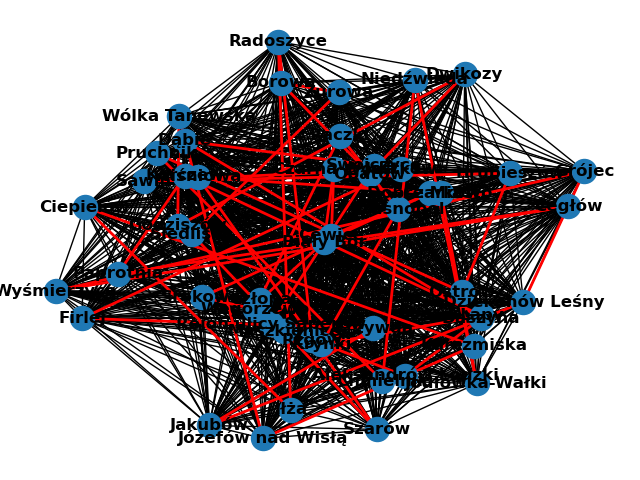
\includegraphics[width=0.8\textwidth]{Chapters/christofides_plot.png}
    \caption{Approximate Tour Path (Christofides Algorithm)}
    \label{fig:christofides_tour}
\end{figure}
\newpage
\section*{ILP Solution}
\begin{center}
    \begin{lstlisting}[language=Python, caption={ILP Solution}]
        # Load data from Excel, setting 'Unnamed: 0' as the index
data_ilp = pd.read_excel(file_path, index_col='Unnamed: 0')

# Extract city names
city_names_ilp = list(data_ilp.columns)
city_indices_ilp = {city: i for i, city in enumerate(city_names_ilp)}

# Extract distances
distances_ilp = {(city_indices_ilp[i], city_indices_ilp[j]): data_ilp.at[i, j] for i in city_names_ilp for j in city_names_ilp if i != j}

# Create optimization model for ILP
model_ilp = LpProblem("TSP", LpMinimize)

# Decision variables for ILP
x_ilp = {(i, j): LpVariable(name=f"x_{i}_{j}", cat='Binary') for i in city_indices_ilp.values() for j in city_indices_ilp.values() if i != j}

# Objective function for ILP
model_ilp += lpSum(distances_ilp[i, j] * x_ilp[i, j] for i in city_indices_ilp.values() for j in city_indices_ilp.values() if i != j), "Minimize Distance"

# Constraints for ILP
# Ensure that each city is visited exactly once
for i in city_indices_ilp.values():
    model_ilp += lpSum(x_ilp[i, j] for j in city_indices_ilp.values() if i != j) == 1, f"VisitOnce_{i}"

# Ensure that each city is left exactly once
for j in city_indices_ilp.values():
    model_ilp += lpSum(x_ilp[i, j] for i in city_indices_ilp.values() if i != j) == 1, f"LeaveOnce_{j}"

# Solve the model and measure execution time for ILP
start_time_ilp = time.time()
model_ilp.solve()
end_time_ilp = time.time()

# Display the results for ILP
print("\nILP Status:", LpStatus[model_ilp.status])

# Print the optimal path for ILP
optimal_path_ilp = [var for var in model_ilp.variables() if var.value() == 1]
print("ILP Optimal Path:")
for var in sorted(optimal_path_ilp, key=lambda v: (int(v.name.split('_')[1]), int(v.name.split('_')[2]))):
    print
    \end{lstlisting}
\end{center}
\subsection*{Results}
ILP Optimal Path
\begin{verbatim}
ILP Status: Optimal
ILP Optimal Path:
Aleksandrów Łódzki Rzgów
.
.
.
.
Łapy Krynki
Żurowa Siedliska
Aleksandrów Łódzki Rzgów
\end{verbatim}

\section*{Comparison with ILP Solutions}

The efficiency and running time of the Christofides algorithm were compared with the optimal ILP solutions obtained in Task 2. A subset of the dataset was chosen for this comparison.
\begin{center}
    \begin{lstlisting}[language=Python, caption={CCompare execution times in a plot}]
        # Display the Exceution time for ILP   
print("Execution Time for ILP:", end_time_ilp - start_time_ilp)

# Display the execution time for Christofides algorithm
print("Execution Time for Christofides:", end_time_christofides - start_time_christofides)

# Compare execution times in a plot
labels = ['ILP', 'Christofides']
execution_times = [end_time_ilp - start_time_ilp, end_time_christofides - start_time_christofides]

plt.bar(labels, execution_times, color=['blue', 'green'])
plt.ylabel('Execution Time (seconds)')
plt.title('Comparison of Execution Times: ILP vs Christofides')
plt.savefig('execution_time_comparison.png')
plt.show()
    \end{lstlisting}
\end{center}
\newpage
\subsection*{Results}
\begin{verbatim}
    Execution Time for ILP: 0.2604055404663086
    Execution Time for Christofides: 0.10591006278991699
\end{verbatim}
\subsection*{Computation Time}

The computation time for both algorithms was recorded and analyzed. Figure \ref{fig:comptime} illustrates the comparison of computation times.

\begin{figure}[H]
    \centering
    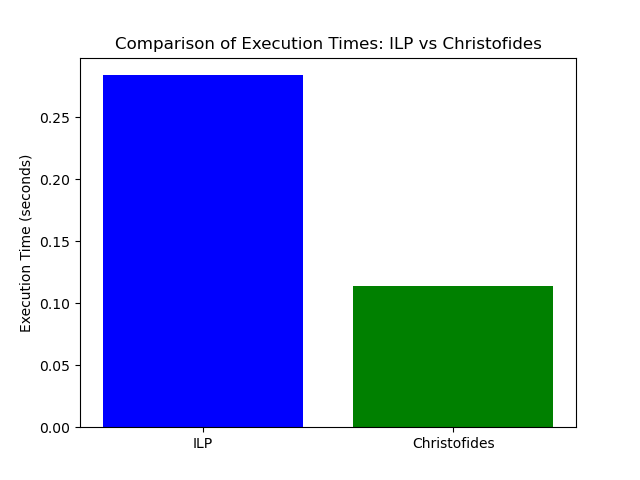
\includegraphics[width=0.8\textwidth]{Chapters/execution_time_comparison.png}
    \caption{Comparison of Computation Time}
    \label{fig:comptime}
\end{figure}

\subsection*{Efficiency Comparison}

The efficiency of the Christofides algorithm was evaluated in terms of the approximation ratio and solution quality compared to the ILP solutions.

\section*{Conclusion}

In conclusion, the Christofides algorithm was successfully implemented and compared with the optimal ILP solutions for the metric TSP. The results provide insights into the trade-off between solution quality and computation time for both approaches.



\begin{thebibliography}{9}
\bibitem{dfj-formulation} Dantzig, G. B., Fulkerson, R. L., \& Johnson, S. M. (1954). Solution of a Large-Scale Traveling-Salesman Problem. \textit{Journal of the Operations Research Society of America}, 2(4), 393–410.

\bibitem{gurobi-example} Gurobi. (n.d.). Traveling Salesman Problem Example. Retrieved from \url{https://colab.research.google.com/github/Gurobi/modeling-examples/blob/master/traveling_salesman/tsp.ipynb#scrollTo=GynJsohc5RvF}
\bibitem{christofides} Christofides, N. (1976). Worst-case analysis of a new heuristic for the travelling salesman problem. \emph{Report 388, Graduate School of Industrial Administration, Carnegie Mellon University}.
\bibitem{ilp_solution} Last Name, First Name. (Year). \emph{Title of the ILP Solution Paper}. Journal Name, Volume(Issue), Page Range. DOI or URL
\end{thebibliography}

% \bibliographystyle{plain}
% \bibliography{Chapters/references}



\end{document}
